\section{Value Atlases: What Only the Cylinder Can Do}\label{sec:atlas}

So far we found each value by hand, one position at a time. With a computer we can instead find the value of
\emph{every} small position and see which values occur at all. We did this twice.
\begin{itemize}
\item \emph{The cylinder atlas} holds every pawn position with at most five pawns on the cylinders
  $\cyl{3},\dots,\cyl{8}$ and the flat boards $\flatb{3},\dots,\flatb{8}$, all with eight ranks:
  $1{,}223{,}689$ positions. They take $10{,}369$ distinct values under the textbook passed-pawn test and
  $10{,}561$ under the e.p.-aware test \lab{C1}; an independent minimax program confirms the textbook outcomes.
\item \emph{The flat census} holds every position with at most six pawns on flat boards of one to four files:
  $231{,}071$ records, standing for $459{,}443$ positions. An independent C solver agrees with ours on every
  record \lab{C2}. We use it for the smallest values (Section~\ref{sec:targets}) and for $\nim{2}$
  (Section~\ref{sec:star2}).
\end{itemize}

\subsection{Which Values Occur}
With at most five pawns, the values without $\pm\BIG$ include the following families.
\begin{itemize}
\item \emph{Nimbers:} only $\star$, and $\nim{2}$ under the textbook test alone (Section~\ref{sec:star2}).
\item \emph{Ups:} ${\uparrow}$, ${\uparrow}\star$, ${\Uparrow}$ and ${\Uparrow}\star$. A single file already holds
  ${\Uparrow}\star$ (Fig.~\ref{fig:basic}(h)).
\item \emph{Fractions:} $\pm1/2$, $\pm1/4$, $\pm3/2$ and $\pm5/2$ on both kinds of board, and $\pm3/4$ only on
  $3$-file cylinders.
\end{itemize}
The six-pawn census adds smaller values, such as $1/8$ and $\upsec\star$ (Section~\ref{sec:targets}).

\begin{figure}[!t]
\centering
\begin{subfigure}[b]{0.36\columnwidth}\centering
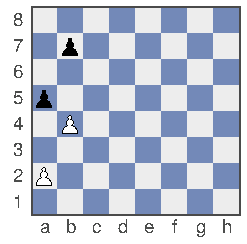
\includegraphics[height=1.25in]{figures/hot3.pdf}
\caption{}
\end{subfigure}\hfill
\begin{subfigure}[b]{0.18\columnwidth}\centering
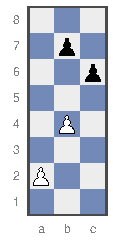
\includegraphics[height=1.25in]{figures/ring3_threequarters.pdf}
\caption{}
\end{subfigure}\hfill
\begin{subfigure}[b]{0.18\columnwidth}\centering
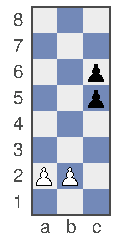
\includegraphics[height=1.25in]{figures/ring3_quarter.pdf}
\caption{}
\end{subfigure}\hfill
\begin{subfigure}[b]{0.22\columnwidth}\centering
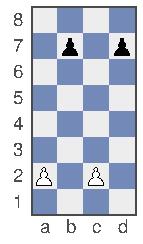
\includegraphics[height=1.25in]{figures/ring4.pdf}
\caption{}
\end{subfigure}
\caption{Hot and cylinder-only pawn values. (a)~White a2, b4 against black a5, b7: $\pm3$, the hottest
position without $\pm\BIG$ (ordinary board; the same on the cylinder). (b)~White a2, b4 against black b7, c6:
$3/4$ (cylinder $\cyl{3}$: files a and c adjacent). (c)~White a2, b2 against black c5, c6: $1/4\pm1/4$
(cylinder $\cyl{3}$). (d)~White a2, c2 against black b7, d7: $\game{3/2\pm1/2}{-3/2\pm1/2}$ under the textbook
test (cylinder $\cyl{4}$: files a and d adjacent).}
\label{fig:hot3}
\end{figure}

\subsection{The Hottest Position}
Apart from $\pm\BIG$, the highest temperature in the atlas (textbook test) is $3$. It is reached by white a2,
b4 against black a5, b7 (Fig.~\ref{fig:hot3}(a)), which is worth $\pm3$ on the ordinary board and on the cylinder
alike \lab{C1}.

Whoever moves first captures. If white (Left) moves first, b4$\times$a5 leaves white's two a-pawns against the lone
black pawn on b7. That pawn is stuck, since either step lets the a5-pawn through, and white is three spare moves
ahead: the value is $3$. If black (Right) moves first, a5$\times$b4 does the same for black and leaves $-3$. Thus
$G=\game{3}{-3}=\pm3$. By Principle~2 (Section~\ref{sec:sums}), this is the first place either player should move.

\subsection{What Only the Cylinder Can Do}
By the cut lemma (Theorem~\ref{thm:cut}), a value that occurs on a cylinder but on no flat board must come from a
\emph{ring}, a position with a pawn on every file. A ring on $n$ files needs at least $n$
pawns, so with five pawns or fewer only $\cyl{3}$, $\cyl{4}$ and $\cyl{5}$ can contribute.

\begin{proposition}[\lab{C1}]\label{prop:cylonly}
Under the textbook test, with at most five pawns, $53$ values free of $\BIG$ occur on some cylinder of width at
most $8$ but on no flat board of width at most $8$. Of these, $40$ come from $3$-file rings and $13$ from $4$-file
rings. Conversely, every value that occurs on a flat board also occurs on some cylinder.
\end{proposition}

Fig.~\ref{fig:hot3}(b)--(d) shows examples. On $\cyl{3}$, white a2, b4 against black b7, c6 is worth $3/4$,
and white a2, b2 against black c5, c6 is worth $1/4\pm1/4$. Both keep their values under the e.p.-aware test.
On $\cyl{4}$, white a2, c2 against black b7, d7 is worth $\game{3/2\pm1/2}{-3/2\pm1/2}$. These are the four
pawns of the $\nim{2}$ candidate of Section~\ref{sec:star2}. On the flat board they make $\nim{2}$ under the
textbook test, and closing the board into a ring turns that into a hot game. Under the e.p.-aware test the
ring is worth $\game{2\pm1}{-2\pm1}$, which is also the e.p.-aware value of the same pawns on the flat board, so
this particular value is no longer cylinder-only.

\subsection{A Correction: Race Rules}
One honest correction. Our first atlas report said that none of the cylinder-only values depends on the race
rule (Section~\ref{sec:rules}). A second, independent computation showed that this is wrong. The $3$-file ring
values do depend on it: $3/4$ becomes $0$ under the mover rule. The $4$-file ring values do not, but they change
when en passant is switched off. So no value is cylinder-only under every combination of race rule and en passant
setting.
